\section{V2}
\subsection{Compiler-Schritte}
\vspace{-0.5cm}
\begin{multicols}{2}
    \begin{minipage}{\linewidth}
        \begin{enumerate}
            \item \textbf{Lexikalische Analyse(scanning):}\newline
                Die Symbole der Sprache werden erkannt und Gruppiert. Leerzeichen werden eliminiert
            \item \textbf{Syntaxanalyse(parsing):}\newline
                 Die erkannten Symbole werden in Sätzen zusammengefasst und in einem Parsbaum dargestellt
            \item \textbf{Semantische Analyse:}\newline
                 Das Quellprogramm wird auf Fehler überprüft (zBsp. Typfehler) und der Parsbaum erhält Informationen über die verwendeten Bezeichner
            \item \textbf{Zwischencode-Erzeugung:}\newline
                 Einige Compiler erzeugen Code in einer Zwischensprache (abstrakte Maschinen)
            \item \textbf{Code-Erzeugung:}\newline
                 Erzeugen von verschiebbarem Maschinencode.      
        \end{enumerate}
    \end{minipage}

    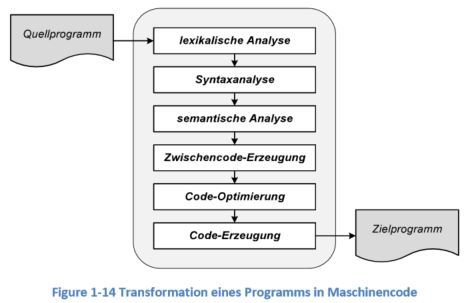
\includegraphics[width=\linewidth]{images/CompilerWorkflow2}
\end{multicols}

\subsection{Busortientierte Systeme}
\subsubsection{Speicher}
\begin{multicols}{2}
    \textbf{RAM}
    \begin{itemize}
        \item Random Access Memory
        \item Schreibe-/Lese-Speicher
        \item Spannungsversorgung erforderlich
        \item für Temporär Daten
    \end{itemize}

    \textbf{ROM}
    \begin{itemize}
        \item Read Only Memory
        \item Festwert Speicher
        \item auch ohne Spg. bleiben Daten erhalten
    \end{itemize}
\end{multicols}

\begin{multicols}{3}
    \begin{minipage}{4cm}
        \textbf{Adressbus}
        \begin{itemize}
            \item unidirektional
            \item bestimmt Grösse des Adressraums
        \end{itemize}
    \end{minipage}
    
    \begin{minipage}{4cm}
        \textbf{Databus}
        \begin{itemize}
            \item bidirektional
        \end{itemize}
    \end{minipage}
    
    \begin{minipage}{5cm}
        \textbf{Steuerbus}
        \begin{itemize}
            \item kontrolliert Buszugriffe
            \item zeitlicher Ablauf der Signale
        \end{itemize}
    \end{minipage}
\end{multicols}

\begin{itemize}
    \item[*] Die gesammte Menge der über den Adressbus adressierbaren Speicherzellen wird \textbf{Adressraum} genannt
    \item[*] Die Anzahl parallel geführten \textbf{Datenleitungen} entspricht der maximal zu übertragenden Datenbreite
    \item[*] Kontrollsigbale werden über den \textbf{Steuerbus} übertragen
\end{itemize}
    \includegraphics[width=0.5\linewidth]{images/SimpleuPSystem}
    
\begin{multicols}{2}    
    \subsubsection{Architectur eines uP}
    \begin{minipage}{1.3\linewidth}
        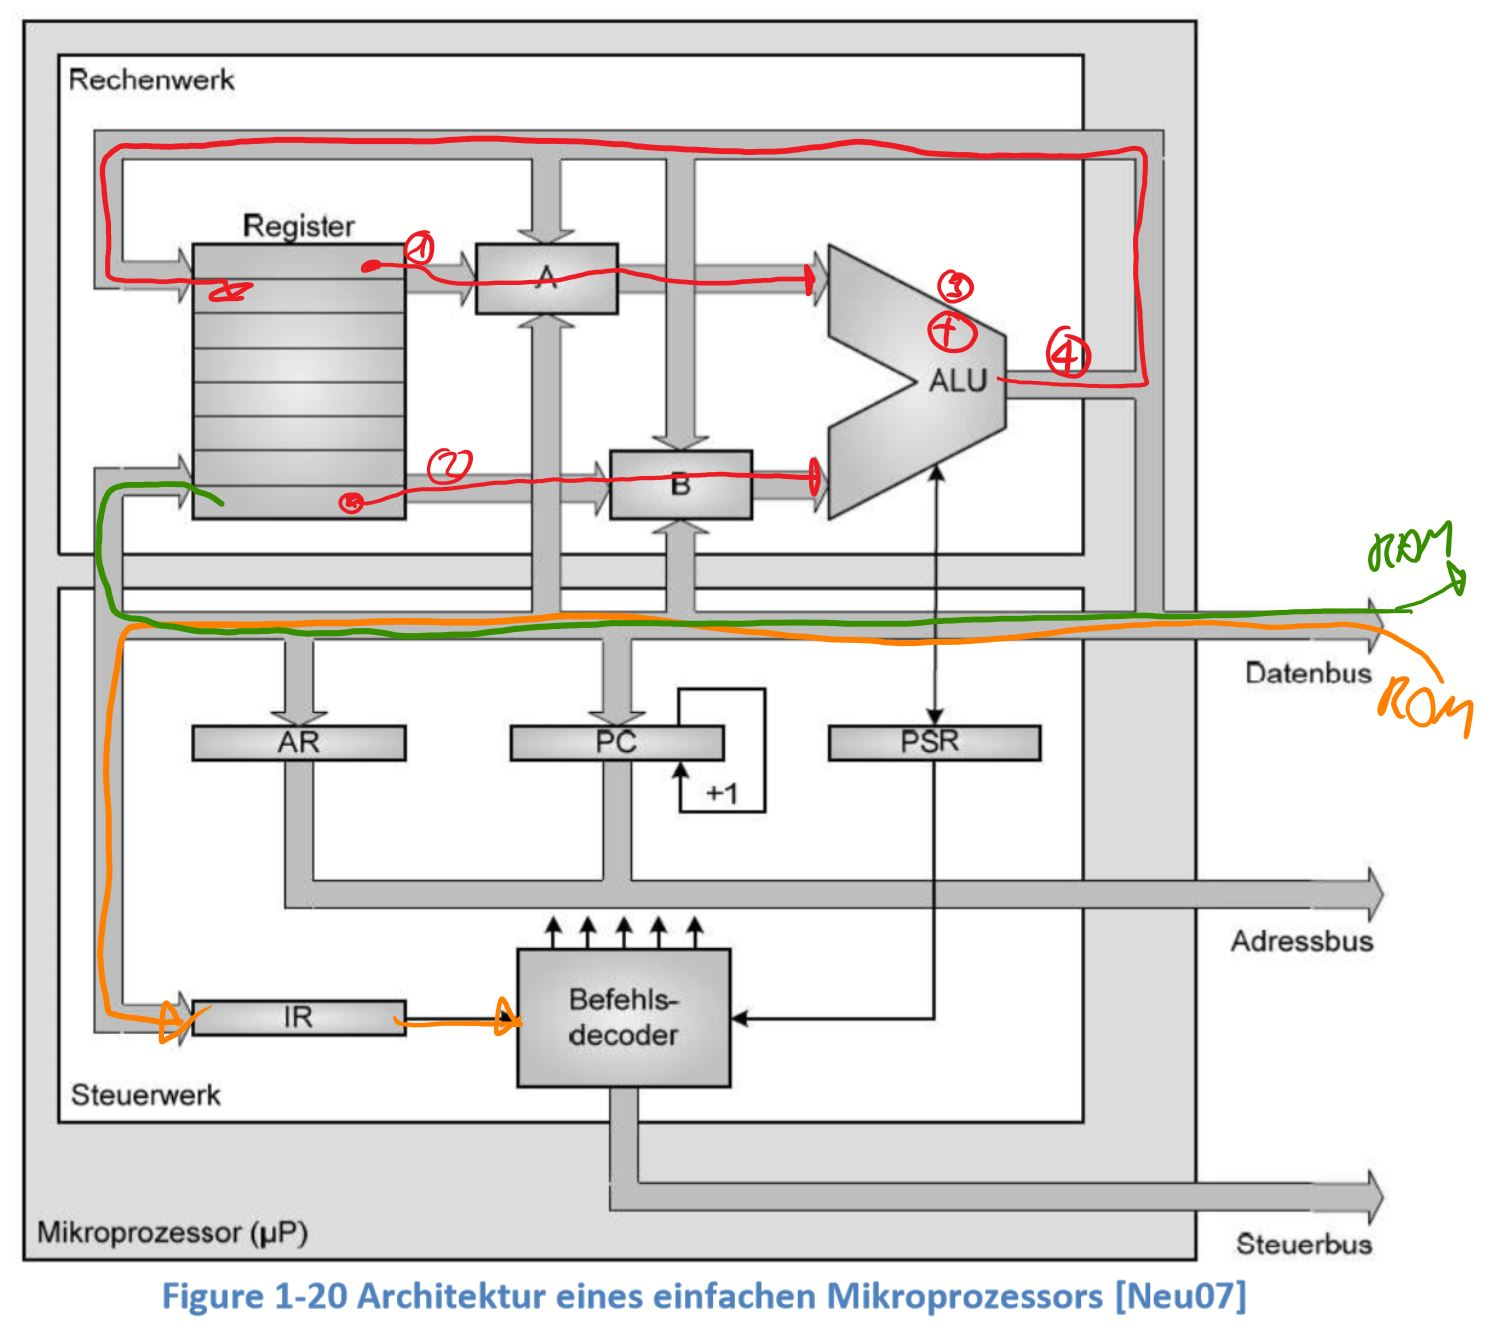
\includegraphics[width=\linewidth]{images/ArchitectuP}
    \end{minipage}
        
    \begin{minipage}[r]{4cm}
        \begin{tabular}[r]{c|c}
            \textbf{AR} & Adressregister  \\ 
            \textbf{PC} & Programm Counter  \\ 
            \textbf{PSR}& Program Status Register \\ 
            \textbf{IR} & Instruction Register  \\ 
        \end{tabular} 
    \end{minipage}
\end{multicols}
    
\begin{multicols}{2}
    \begin{minipage}{8cm}
        \textbf{Flags}\newline
        \begin{tabular}{|c|c|l|}
            \hline 
            \textbf{N}  &\textbf{Negative}  & Das von der ALU berechnete Ergebniss ist negativ \\ 
            \hline 
            \textbf{Z}  &\textbf{Zero}      & Das von der ALU berechnete Ergenis ist gleich \textbf{0} \\ 
            \hline 
            \textbf{C}  &\textbf{Carry}     & Die Berechnung der ALU hat zu einem Übertrag geführt  \\ 
            \hline 
            \textbf{V}  &\textbf{Overflow}  & Die Berechnung der ALU hat zu einem Overflow geführt  \\ 
            \hline 
        \end{tabular} 
    \end{minipage}
\end{multicols}

\subsection{Befehlszyklus}
    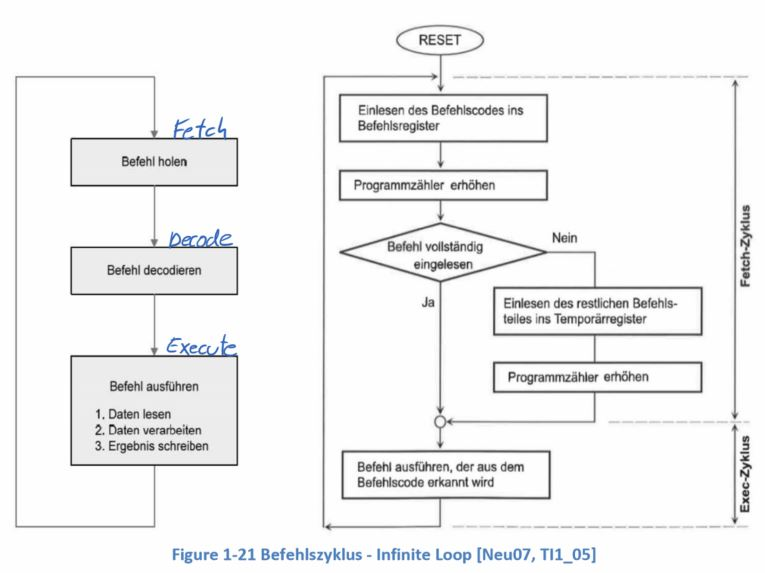
\includegraphics[height=9cm]{images/CommandFlowChart}
